%%%%%%%%%%%%%%%%%%%%%%%%%%%%%%%%%%%%%%%%%%%%%%%%%%%%%%%%%%%%%%%%%%%%%
\subsection{Amortizing Iteration Latency with Batching (8 marks)}
\label{sec:1d}
%%%%%%%%%%%%%%%%%%%%%%%%%%%%%%%%%%%%%%%%%%%%%%%%%%%%%%%%%%%%%%%%%%%%%


The result is reported in \autoref{tab:float-summary} as well as \autoref{fig:amortizing}.
The usage of BRAM\_18K exceeds 100\% when the batch size comes to \texttt{512}.
When the batch size is \texttt{256}, the BRAM\_18K usage is 60\%, which achieves the goal of 55\%.
The corresponding latency is 57103 cycles.

In order to evaluate its efficiency, an additional baseline with the batch size 256 and without any optimization is conducted.
The result shows the baseline took 29020446 cycles, which is 508x longer than the optimized one.

It can also be evaluated by calculating the average latency per input.
In baseline\footnote{Partition (\texttt{dim}=2, \texttt{factor}=16)}, the batch size is 8 and the latency per input is 534.9 cycles.
This design's latency per input is 223.1 cycles, a 2.4x improvement.

\begin{figure}
    \centering
    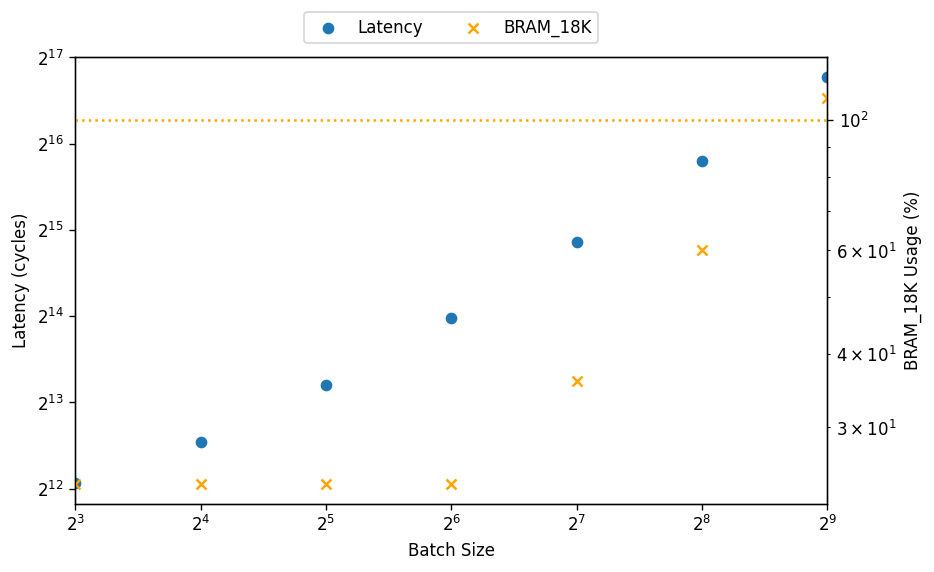
\includegraphics[scale=0.64]{images/amortizing.png}
    \caption{Latency and BRAM\_18K usage}
    \label{fig:amortizing}
\end{figure}
